\chapter{\ak\ Synchroniser}\label{chap_impl}
In this chapter we describe the source language for an \ak\ synchroniser and its implementation. Prior to describing the language in details, we present a mathematical model of a synchroniser from \cite{astrakahn} and outline sources of non-determinism in synchronisers.

The $aksync$ compiler is integrated into the current \ak\ runtime system prototype. It takes the source code of a synchroniser program, performs the syntactic and semantic analysis of it, builds a synchroniser object and generates the CAL passport of the synchroniser.


    \section{Mathematical Model}
From the mathematical point of view a synchroniser is a pair
\begin{equation}
(\Phi, \; \Pi),\\\nonumber
\end{equation}
where $\Phi = (A, \; S, \; T)$ is a nondeterministic state machine with the alphabet of events $A \subseteq C \times P$, where $C$ denotes the set of input channels and $P$ the set of the predicates on channel messages\footnote{An event $(c, \; p) \in A$ represents the reception of a message on channel $c$ that satisfies the predicate $p$}. The set of abstract states in $\Phi$ is denoted as $S \supseteq \{s_{0}\}$ with the start state $s_{0}$, $T \: : \: A \times S \to S$ is the transition matrix of $\Phi$. The path functional $\Pi \: : \: S \times \Omega \to V^{(*)}$ defines the output of the synchroniser, where $\Omega$ is the set of output channels and $V$ is the set of message values\footnote{$V^{(*)}$ denotes a set of all sequences from $V$}.

In state $s_{k}$ the functional is based on the retrospective sequence of transitions from the most recent visit to the start state $s_{0}$ to $s_{k}$:
\begin{equation}
(s_{0}, c_{0}), \: (s_{1}, c_{1}),... \: (s_{k}, c_{k}),\\\nonumber
\end{equation}
where $c_{i} \in C$, $0 \le i \le k$ is the channel that caused the transition from the state $s_{i}$.

Let $\mu_{i}$ be the message received in the transition from the state $s_{i}$. Then
\begin{equation}
\Pi \; (s_{k}, \omega_{m}) = \psi_{\sqcap} \; \{\mu_{i} \: | \: \rho_{ki}^{m} \; (s_{i}), \: 0 \le i \le k\},\\\label{predic}
\end{equation}
where $\rho_{ki}^{m}$ is the selection predicate that defines $\Pi$, and $\psi_{\sqcap}$ is the operator that coerces the messages in the operand set to their joint greatest subtype.

From the above, the synchroniser is fully defined by two functions:
  \begin{enumerate}
  \item The transition matrix $T$

The state machine can have a regular structure whereby many transitions can be defined at once by a formula with some limited-range integer variables. For example, a machine with 8 states could have a transition matrix defined thus: $S_{k \; mod \; 8} \to S_{k+1 \; mod \; 8}$. In order to be able to employ regular transition graphs, \ak\ allows synchronisers to declare \emph{state} variables.

\textbf{Example: the counter synchroniser}  Counter sends every $n$-th message from its input channel to the output channel, other messages are disregarded. The transition diagram for the counter synchroniser for $n = 3$ is given in Figure \ref{fig:counter}.a.

The counter synchroniser is a pair $(\Phi, \; \Pi)$, where
  \begin{itemize}
  \item[] $\Phi = (A, \; S, \; T)$,
    \begin{itemize}
    \item[] $C = (a)$, $P = (true)$, $A = C \times P = ((a, \; true))$,
    \item[] $S = (s_{0}, \; s_{1}, \; s_{2})$, $s_{0}$ -- start state,
    \item[] $T$:
      \begin{tabular}{c|c|c|c}
      $A$ \textbackslash $S$ & $s_{0}$ & $s_{1}$ & $s_{2}$\\
      \hline
      $(a, \; true)$ & $s_{1}$ & $s_{2}$ & $s_{0}$\\
      \end{tabular}
    \end{itemize}
  \item[] $\Pi \: : \: S \times \Omega \to V^{(*)}$,
    \begin{itemize}
    \item[] $\Omega = (c)$,
    \item[] $V = (a)$
    \end{itemize}
  \end{itemize}

An output message is emitted when a transition happens from the state $s_{2}$. This state is reached in a single path:
  \begin{itemize}
  \item[]
$W_{0} = ((s_{0}, \; a), \: (s_{1}, \; a), \: (s_{2}, \; a))$
% fixed rho{1i}^{c} to rho{2i}^{c}
$\Pi \; (s_{2}, c) = \psi_{\sqcap} \; \{\mu_{0} = a \: | \: \rho_{20}^{c} \; (s_{0}) = 0, \mu_{1} = a \: | \: \rho_{21}^{c} \; (s_{1}) = 0, \mu_{2} = a \: | \: \rho_{22}^{c} \; (s_{2}) = 1\}$, $k = 1$, $i = 0,1,2$ 
  \end{itemize}

The state machine behind the counter has a regular structure, and for this synchroniser all its transitions can be defined with a single formula: $S_{k \; mod \; 3} \to S_{k+1 \; mod \; 3}$. Considering this, the transition matrix $T$ would be:
  \begin{tabular}{c|c}
  $A$ \textbackslash $S$ & $S_{k \; mod \; 3}$\\
  \hline
  $(a, \; true)$ & $S_{k+1 \; mod \; 3}$
  \end{tabular}

Some possible transition diagrams of the counter synchroniser are given in Figure \ref{fig:counter}. The diagram \ref{fig:counter}.a represents the unrolled regular structure of the synchroniser. However, this representation is inconvenient when $n \gg 1$. The diagram can be folded using state variables. Two possible variants are shown in figures \ref{fig:counter}.b and \ref{fig:counter}.c. The state variable $c$ acts as an induction variable in a while loop with the exit condition $c \ge 3$.

  \begin{figure}[here]
  \centering
  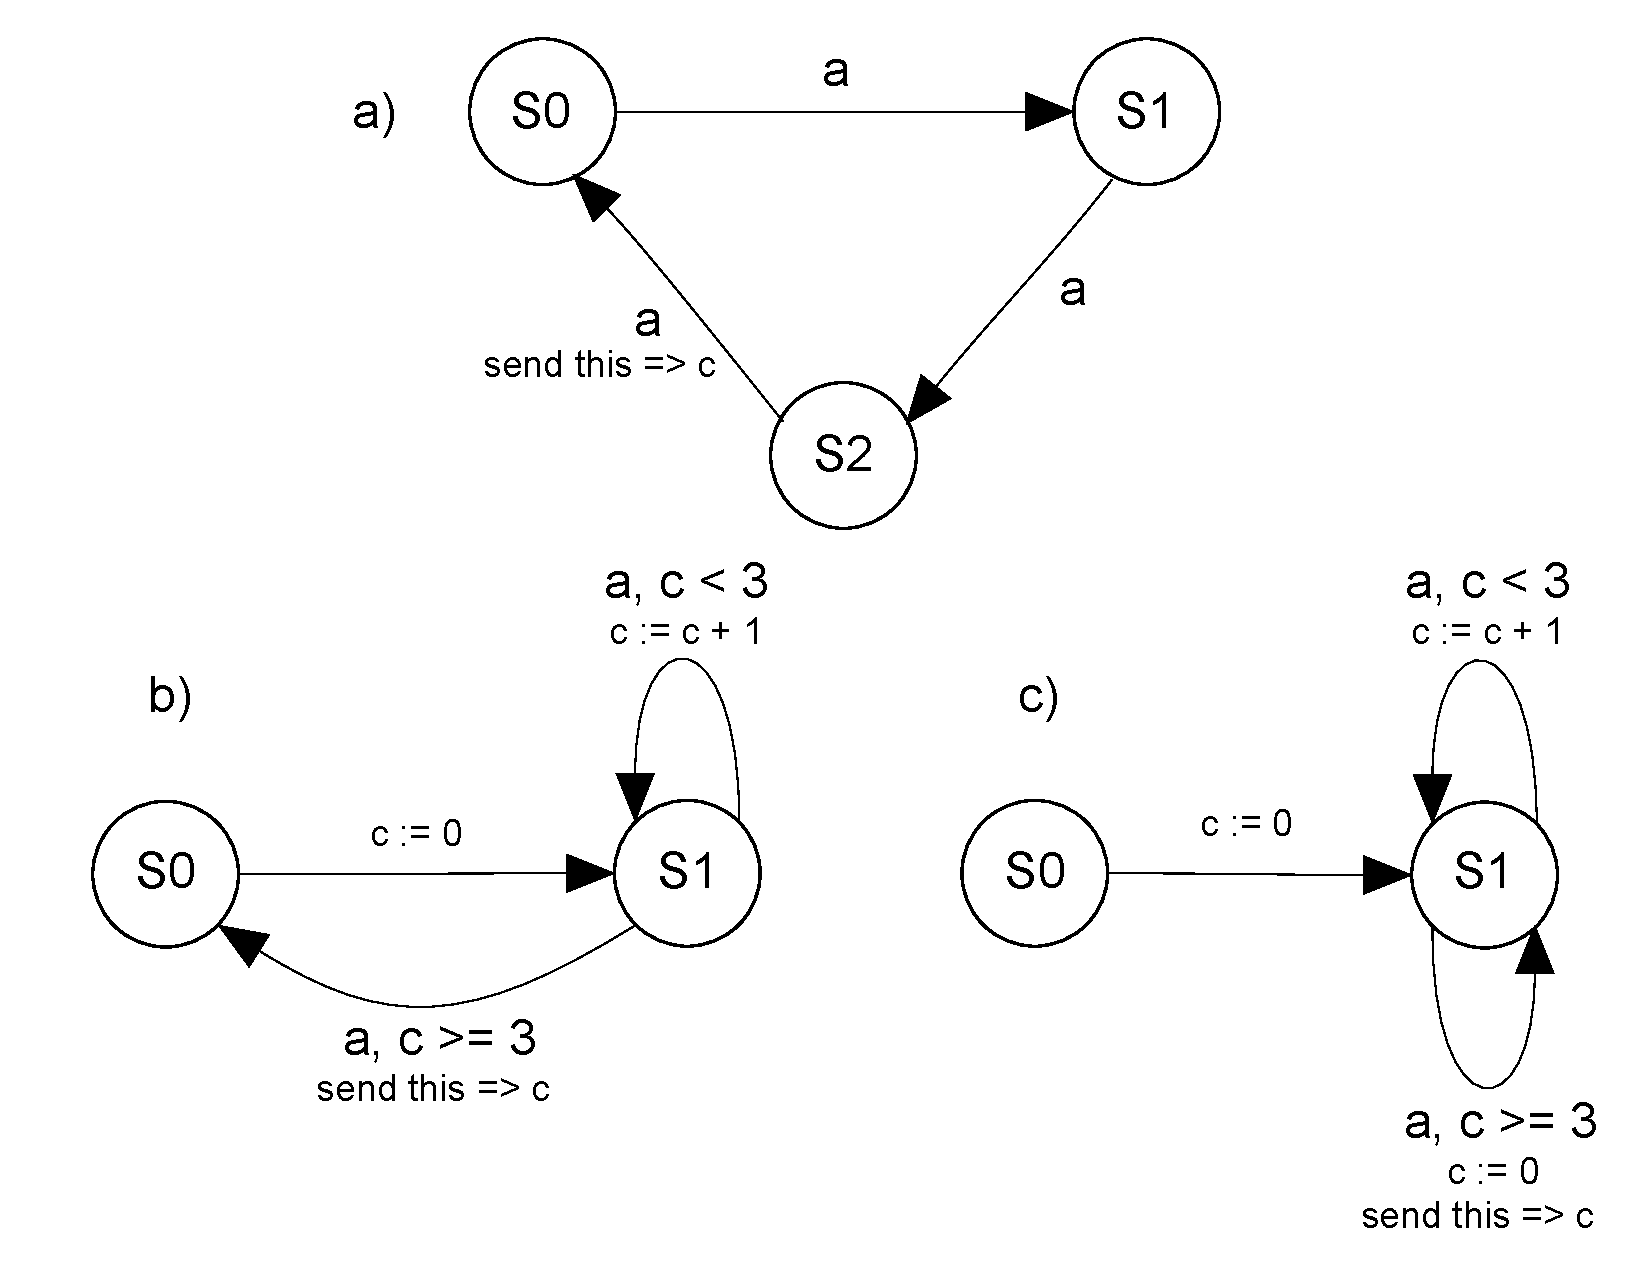
\includegraphics[scale=0.4]{figs/counter.pdf}
  \caption{The transition diagrams of the counter synchroniser}
  \label{fig:counter}
  \end{figure}


  \item The selection predicate $\rho$ (see formula \ref{predic})

In a given state $k$ for each output channel $\omega_{m}$ we note all $i$ on which $\rho_{ki}^{m}$ is true. Those message values must be saved in a previous state and recalled in state $k$. The functional $\Pi$ can be implemented as function that retrieves all the saved messages at once; however, it is expected that the boolean vector $\omega_{i} = \rho_{ki}^{m}$ has only very few true elements. Consequently it is feasible to implement the storage mechanism that \ak\ provides for synchronisers in the form of individual \emph{store} variables. The type of a store variable is determined when a variable is assigned.

\textbf{Example: the binary zip synchroniser}  Zip2 receives messages on its input channels and sends their concatenation to the output channel. In the resulting concatenation there is exactly one message from each input channel and those messages are combined for the output.

The zip2 transition diagram is given in Figure \ref{fig:zip2}. The message received in the current transition is referred by a keyword \emph{this}. $ma$ and $mb$ are the store variables associated with the input channels $a$ and $b$ respectively. The statement \emph{send} indicates the sending of a message to an output channel.

  \begin{figure}[here]
  \centering
  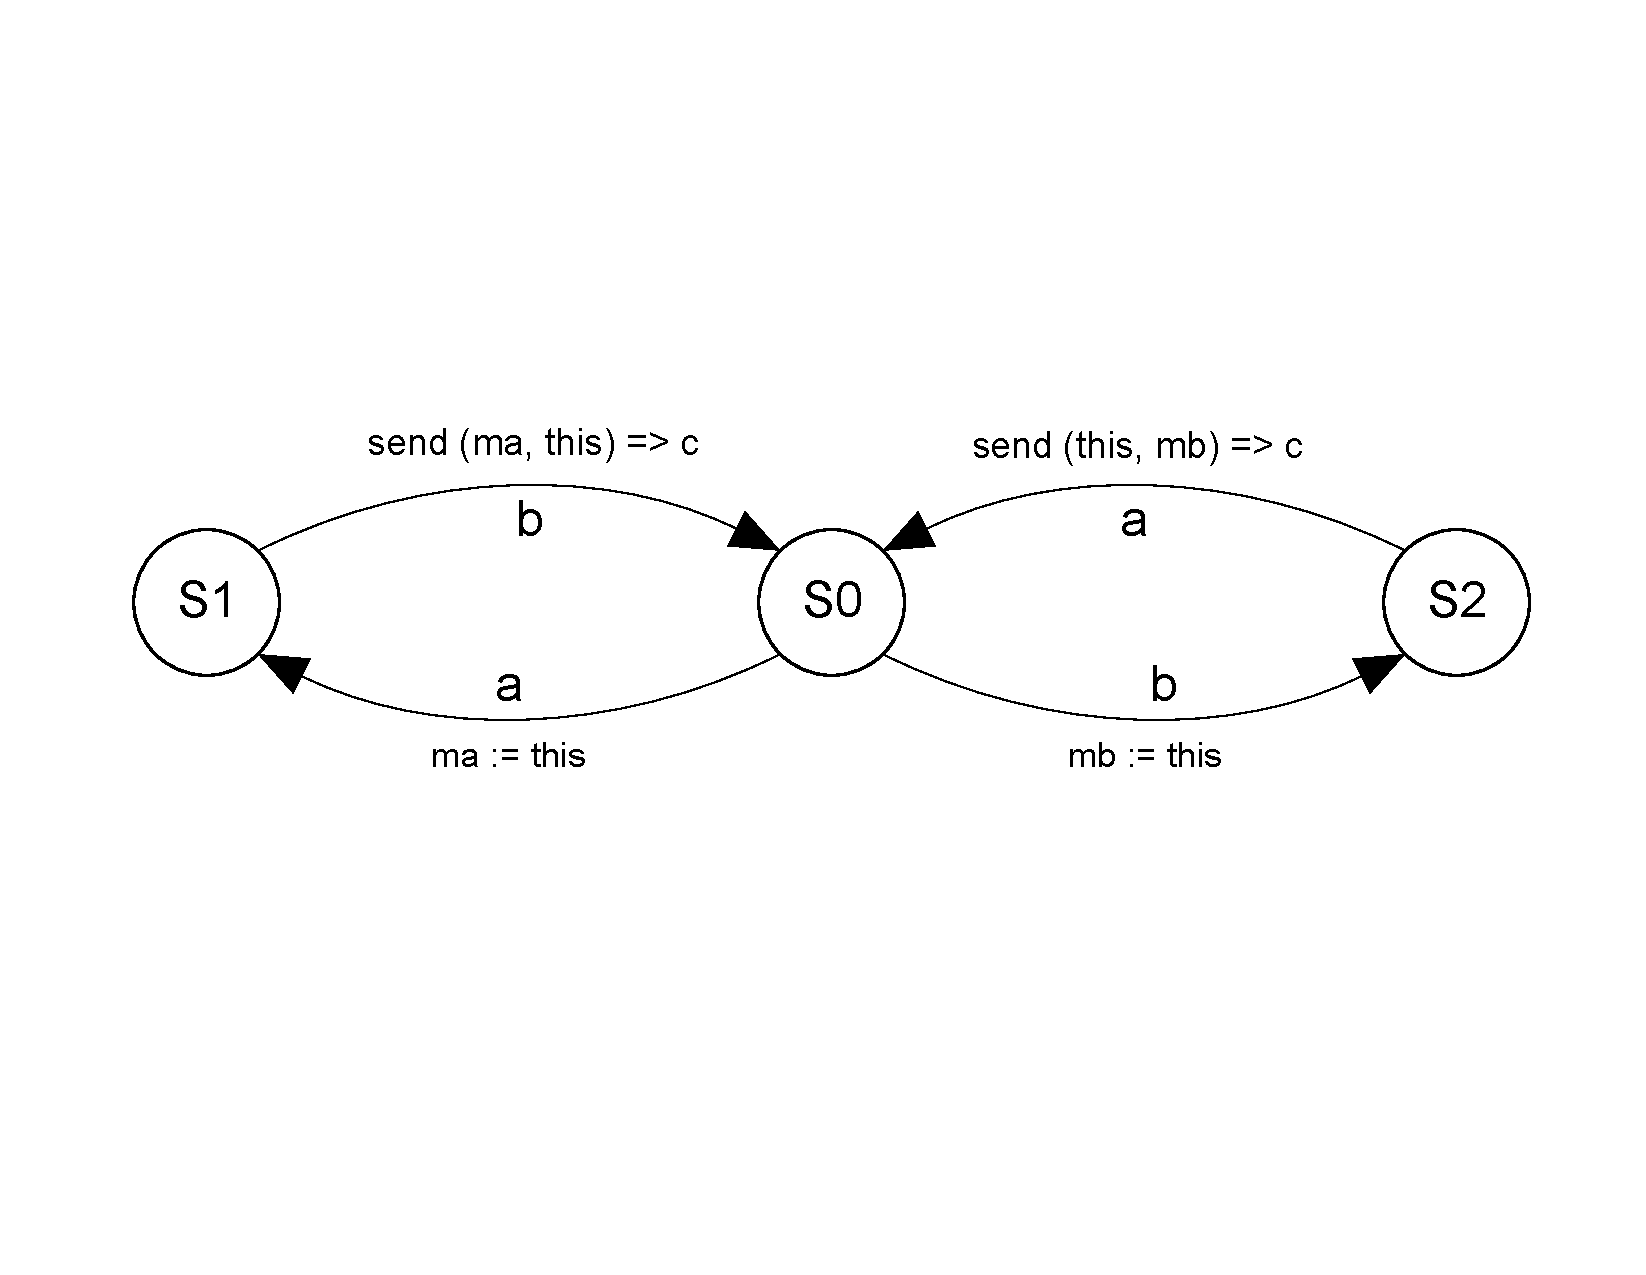
\includegraphics[scale=0.4]{figs/zip2.pdf}
  \caption{The transition diagram of the zip2 synchroniser}
  \label{fig:zip2}
  \end{figure}

Mathematically, the zip2 synchroniser is a pair $(\Phi, \; \Pi)$, where
  \begin{itemize}
  \item[] $\Phi = (A, \; S, \; T)$,
    \begin{itemize}
    \item[] $C = (a, \; b)$, $P = (true)$, $A = C \times P = ((a, \; true), \: (b, \; true))$,
    \item[] $S = (s_{0}, s_{1}, s_{2})$, $s_{0}$ -- start state,
    \item[] $T$:
      \begin{tabular}{c|c|c|c}
      $A$ \textbackslash $S$ & $s_{0}$ & $s_{1}$ & $s_{2}$\\
      \hline
      $(a, \; true)$ & $s_{1}$ & $s_{1}$ & $s_{0}$\\
      \hline
      $(b, \; true)$ & $s_{2}$ & $s_{0}$ & $s_{2}$\\
      \end{tabular}
    \end{itemize}
  \item[] $\Pi \: : \: S \times \Omega \to V^{(*)}$,
    \begin{itemize}
    \item[] $\Omega = (c)$,
    \item[] $V = ((a, \; b))$
    \end{itemize}
  \end{itemize}

An output message is emitted when a transition happens either from state $s_{1}$ or state $s_{2}$. These states are reached in two paths:
  \begin{itemize}
  \item[]
$W_{0} = ((s_{0}, \; a), \: (s_{1}, \; b))$

$\Pi \; (s_{1}, c) = \psi_{\sqcap} \; \{\mu_{0} = a \: | \: \rho_{10}^{c} \; (s_{0}) = 1, \mu_{1} = b \: | \: \rho_{11}^{c} \; (s_{1}) = 1\}$, $k = 1$, $i = 0,1$
  \item[]
$W_{1} = ((s_{0}, \; b), \: (s_{2}, \; a))$

$\Pi \; (s_{2}, c) = \psi_{\sqcap} \; \{\mu_{0} = b \: | \: \rho_{20}^{c} \; (s_{0}) = 1, \mu_{2} = a \: | \: \rho_{22}^{c} \; (s_{2}) = 1\}$, $k = 2$, $i = 0,2$ 
  \end{itemize}
  \end{enumerate}

So far we have given a formal definition of the synchroniser. Along with it we have introduced two important concepts for the synchroniser that are considered as a part of the synchroniser language. First is a message storage mechanism we call a store variable. Second is a mechanism for defining large regular transition matrices, which we call a state variable.


\section{The Language of \ak\ Synchronisers}
The \ak\ synchroniser is a finite state machine, therefore the basic building blocks of a synchroniser program are states and transitions. A state of a synchroniser is fully defined by the corresponding state of the finite state machine and the values of the state variables. A transition is the act of moving to another state which is initiated by a triggering event. A triggering event for the synchroniser transition is the arrival of a message to the associated channel. The message may be required to have a specific structure. In addition, a transition may be guarded by special conditions on state variable values. If the condition is satisfied the transition fires, otherwise it is cancelled.

Once a transition is known to fire, optional actions may be performed before the underlying state machine makes the move. These actions include changing the state and store variables and sending messages to output channels. In order to change the state and store variables, the synchroniser language provides state and store expressions over them.

This section gives an overview of the \ak\ synchroniser programming language. The formal grammar of the \ak\ synchroniser is provided in Appendix \ref{sync_syntax}.

  \subsubsection*{Program structure}
A synchroniser program consists of a header followed by a body wrapped in braces. The begining of a synchroniser program is indicated by the keyword $synch$.

The header contains the synchroniser's name and the channel signature. The name is an ASCII string that follows the C convention.

The body lists the state and store variable declarations and the states of the underlying finite state machine. Each state is supplemented by a list of transitions. Each transition declares its triggering condition which includes an optional guarding state expression, an optional list of actions, and, finally, the destination state.


% We removed macros from the language. The compiler must invoke a preprocessor to expand them.
  \subsubsection*{Channel signature}
The channel signature defines the input and output channels of the synchroniser and their bracketing depths. The synchroniser header (Fig. \ref{min_sync_head}) declares the synchroniser $min$ with two input channels that are connected to the ports $a$, $b$ and two output channels that are connected to the ports $c$, $d$. If the bracketing depths of the channels are not specified, they are assumed to be 0. Thus, the bracketing depth of the channel $a$ is 0.

The input channel depth $-1$ indicates that the input channel is ignored in the synchroniser program. The output channel with the depth $-1$ must not have data sent to them.

\begin{figure}[h!]
\begin{lstlisting}[frame=single]
synch min (a, b:p | c:2, d:p+1)
\end{lstlisting}
\caption{The synchroniser header}
\label{min_sync_head}
\end{figure}

%% TODO remove read-only state variables

The \ak\ synchroniser allows one to declare constant and configurable integer depths for the input and output channels. In addition, the depth of an output channel can be specified with an integer shift to the configurable input channel depth.

The input channels are required to have the bracketing depths specified in the signature. Thus, the channel $a$ (i.e. the channel connected to the port $a$) of $min$ must have zero bracketing depth. The channel $b$ has a configurable bracketing depth $p$. The actual values of configurable bracketing depths of input channels are determined by the \ak\ compiler by tracing bracketing depth relations over the application network.

The output channels of a synchroniser are guaranteed to have the bracketing depths specified in its channel signature. Thus, the synchroniser $min$ must send messages to the output channel $c$ at depth 2. The output channel $d$ must have the bracketing depth $p+1$, i.e. the depth of the input channel $b$ plus 1.


%% The width of int type is declared explicitly to reduce the number of potential states of automata.
  \subsubsection*{Variable declaration}
%% TODO! Add about state and store variables initialisation.
%% state int(8) a, b=1, c=8; // assignes a=0 b=1 c=9
%% enum (a,b,c) foo, bar=a;  // assignes foo=0 bar=a
The start of a state variables declaration is marked by the keyword $state$. A state variable may be either an unsigned integer of some size or a C-style enumeration. State and store variable names are user-defined indentifiers. A user-defined identifier is an ASCII string that follows the C convention.

Line 1 in Fig. \ref{sync_statevar} declares state variables $a$, $b$, $c$ of size 4. Thus, all three variables are declared to have integer values in the range $[0; 15]$. Generally, a state variable of size $n$ has integer values in the range $[0; 2^{n}-1]$. State variable $c$ is initialised with an integer value 0.

The state variable $foo$ that is declared on the line 2 in Fig. \ref{sync_statevar} can only be assigned the values $d$, $e$ and $f$ specified in the enumeration. The enumeration values are integer constants. If they are not specified explicitly, they are assigned consequtive positive integers starting with 0.
%The width of the $int$ type is $\lceil \log_{2}{n} \rceil + 1$, where $n$ is the number of values in the enumeration.
Thus, the variable $foo$ has integer values $d=0$, $e=1$ and $f=2$. % of the width $\lceil \log_{2}{3} \rceil + 1 = 3$. If the values are specified explicitly, the width is determined as $\lceil \log_{2}{(m+1)} \rceil + 1$, where $m$ is the biggest value in the enumeration. For the variable $bar$ declared in line 3 of Fig. \ref{sync_statevar} $m=4$ and the width is $\lceil \log_{2}{(5)} \rceil + 1 = 4$.


The values can be specifed explicity (see line 3 in Fig. \ref{sync_statevar})

Integer state variables and enum values can be mixed freely in state expressions. Enum values are interpreted as integer constants.%read-only integer state variables. % constant integers!

\begin{figure}[h!]
\lstset{numbers=left, numberstyle=\small, stepnumber=1, numbersep=8pt}
\begin{lstlisting}[frame=single]
state int(4) a, b, c = 0;
state enum(d, e, f) foo;
state enum(x = 1, y = 2, z = 4) bar;
store msg_a, msg_b;
\end{lstlisting}
\caption{State and store variables declaration}
\label{sync_statevar}
\end{figure}

A store variable declaration begins with the keyword $store$. Line 4 in Fig. \ref{sync_statevar} declares state variables $msg\_a$ and $msg\_b$. Store variables do not need an explicit type specification; their types are determined on the first assignment to the variable.

All the state and store variables are global to all the states.


  \subsubsection*{States and transitions}
States and transitions of the synchroniser define which channels are read and in what order. Fig. \ref{zip_struc} presents the code of the binary zip synchroniser's state machine. Line 1 declares the start state of the synchroniser. The $on$ clause indicates the beginning of the transition list. In the start state the zip2 synchroniser acceptes messages from both input channels $a$ and $b$. State and store expressions associated with the transition and the destination state are specified in the braces.

\begin{figure}[h!]
\lstset{numbers=left, numberstyle=\small, stepnumber=1, numbersep=8pt}
\begin{lstlisting}[frame=single]
start {
  on:
    a { goto s1;    }
    b { goto s2;    }
}
s1 {
  on:
    b { goto start; }
}
s2 {
  on:
    a { goto start; }
}
\end{lstlisting}
\caption{State machine of the zip2 synchroniser}
\label{zip_struc}
\end{figure}

When the zip2 synchroniser is in the start state and it receives a message from channel $a$, the underlying state machine transitions to state $s1$. In this state the synchroniser can only receive messages from channel $b$ since there's no transition triggered by channel $a$ and defined in this state. When the message on channel $b$ is received, the state machine transitions to the start state. Lines 10-13 define similar behaviour in state $s2$.

%% Change 'scopes'. 'Blocks' probably
The synchroniser language supports top-down prioritised transition scopes. They are marked by the $elseon$ keyword. A synchroniser in state $foo$ in Fig. \ref{sync_scope} acceptes messages from channels connected to the ports $a$, $b$, $c$ and $d$. When no destination state is specified for a transition, a synchroniser transitions to the current state. If all channels are ready at the same time in state $foo$, the synchroniser processes messages from either channel $a$ or $b$ first. When all messages from channels $a$ and $b$ are processed the synchroniser receives messages from channel $c$. If there're no messages in channels $a$, $b$ and $c$ the synchroniser receives messages from channel $d$.

\begin{figure}[h!]
\lstset{numbers=left, numberstyle=\small, stepnumber=1, numbersep=8pt}
\begin{lstlisting}[frame=single]
foo {
  on:
    a { }
    b { }
  elseon:
    c { }
  elseon:
    d { }
}
\end{lstlisting}
\caption{Prioritised transition scopes}
\label{sync_scope}
\end{figure}


  \subsubsection*{State expressions}
A state expression is a combination of integer constants, state variables and operators, which defines an integer value. The interpretation of a state expression follows the C rules of precedence and association. State expressions can be assigned to state variables. Under the assumption that the output channel has the infinite capacity a synthetic example in Fig. \ref{sync_state_exp} counts the number of messages received from channel $a$ between the arrivals of messages in channel $b$. Line 1 declares the 8-bit integer $count$ and initialises it with 0. When a message from $a$ is received the value of $count$ increases by 1 (see line 5).

\begin{figure}[h!]
\lstset{numbers=left, numberstyle=\small, stepnumber=1, numbersep=8pt}
\begin{lstlisting}[frame=single]
state int(8) count = 0;
foo {
  on:
    a {
      set count = [count + 1];
    }
  elseon:
    b {
      set n = [count], count = [0];
      send count:[n] => c;
    }
}
\end{lstlisting}
\caption{Use of state variables and expressions}
\label{sync_state_exp}
\end{figure}

When a message from channel $b$ is received the value of $count$ is stored in the temporary variable $n$, set to 0 and then $n$ is sent to the output channel.

The variable $n$ does not have to be declared and is considered an alias for the integer expression. Temporary variables are available until the state machine of a synchroniser makes the next transition.


  \subsubsection*{Triggering of a transition}
The channel name on its own stands for the availability predicate for the corresponding channel, i.e. the condition that a message of any kind is available. Whether a transition takes place depends on the channel status and optionally the content of the message.

When a message is received on a channel, it can be matched with a pattern in order to extract parameters needed to select a specific transition. Line 3 of Fig. \ref{sync_trans} checks whether a message received from the input channel $a$ is a unique choice. Then the one and only variant is checked on whether it contains the label $x$. If it does, the value of $x$ is stored in a temporary variable $x$. The tail of the message, i.e. all label-value pairs except for the value labeled $x$, is stored in a temporary variable $t$. Both $x$ and $t$ are available until the state machine makes the next transition.

\begin{figure}[h!]
\lstset{numbers=left, numberstyle=\small, stepnumber=1, numbersep=8pt}
\begin{lstlisting}[frame=single]
foo {
  on:
    a.(x || t)  { }
    a.?v        { }
    a.?v(x, y)  { }
    a.@[k]      { }
}
\end{lstlisting}
\caption{Message content extraction}
\label{sync_trans}
\end{figure}

To support message formats where several variants of a message are possible, a qualifier \begin{bf}?\end{bf}$\alpha$ is available as an input condition. It qualifies input messages as belonging to the $\alpha$ variant. Line 4 of Fig. \ref{sync_trans} checks whether the message received from channel $a$ contains the variant $v$. Line 5 checks whether the message that contains the variant $v$ with only two fields labeled $x$ and $y$. 

A channel carries a stream that consists of messages and possibly segmentation marks. Line 6 in Fig. \ref{sync_trans} checks if the message is a segmentation mark of the depth equal to $k$. The depth of a segmentation mark can be compared with a state expression.

Several different channels can be tested in any given state, however, once the readiness of a channel is established, the synchroniser is committed. Hence the set of conditions applied to the message on any input channel must be exhaustive. In Fig. \ref{sync_trans} it is not, because there is no pattern for messages that do not contain the field label $x$, the variant $v$ and are not a segmentation mark of depth $k$ at the same time. In this case the final clause $a$\begin{bf}.else;\end{bf} is assumed. This clause discards the input message and transitions the synchroniser back to its current state.

A transition can be guarded by a state expression. In this case the transition fires only if the guarding expression evaluates to true. The synchroniser in Fig. \ref{sync_g_state_exp} sends every 256-th message to the output channel. Line 1 declares the 8-bit state variable $i$ and initialises it with 0. The variable is incremented every time a message from channel $a$ is received, except when it reaches 255, in which case it is reset to 0 and the received message is sent down channel $c$. 

Values that are matched from the message can be used in guarding state expressions.
\begin{figure}[h!]
\lstset{numbers=left, numberstyle=\small, stepnumber=1, numbersep=8pt}
\begin{lstlisting}[frame=single]
state int(8) i;
start {
  on:
    a & [i < 255] {
      set i = [i + 1];
    }
    a & [i = 255] {
      set i = [0];
      send this => c;
    }
}
\end{lstlisting}
\caption{Use of guarding state expressions}
\label{sync_g_state_exp}
\end{figure}


  \subsubsection*{Store expressions and sending messages}
%% TODO Probably fix it after writing about CAL terms.
Store expression is a mechanism to combine data. In \ak\, data are typed. Types are CAL terms. The result of the store expression can be either saved in a store variable or sent down an output channel.

The example in Fig. \ref{sync_send} demonstrates the use of store expressions and the $send$ clause. In the start state the synchroniser receives messages from channel $a$ that has the label $n$ in it. Line 5 increments the value under the label $n$ and stores it in the store variable $ma$ under the label $n$ together with the tail $t$. The operator $'$ applied to the variable $x$ creates the record $'x': value(x)$. This is a shorthand useful for the avoidance of tedious notation.

%% TODO Provide a more convincing example for 'id and this
\begin{figure}[h!]
\lstset{numbers=left, numberstyle=\small, stepnumber=1, numbersep=8pt}
\begin{lstlisting}[frame=single]
store ma;
start {
  on:
    a.(n || t) {
      set ma = (n:[n+1] || t);
      goto s1;
    }
}
s1 {
  on:
    b {
      send ma || this => c;
      goto start;
    }
}
\end{lstlisting}
\caption{Use of store expressions and the $send$ clause}
\label{sync_send}
\end{figure}

A message received on a channel is referred to by the keyword $this$ within the active transition. In state $s1$ the synchroniser receives messages from channel $b$. When a message is received, it is concatenated with the store variable $ma$ (see line 12) and sent to the output channel $c$.


\section{Execution Order of Synchroniser\label{execod}}
In order to achieve the lowest latency, an \ak\ synchroniser exploits a non-deterministic behaviour. In a certain state more than one input channel may be ready, however, a state machine receives one input message at a time. The synchroniser does not take any transition that potentially causes sending to a blocked channel. Of the transitions that do not send to blocked channels, which one will be triggered is defined by the fairness policy: when more than one transition is possible in a given state, all choices will be made with the same frequency. If transitions are prioritised, the choices are made within each scope at first.

Once the transition has been taken and the associated actions have been executed, the synchroniser transitions to the destination state. In order to avoid transitioning to a state in which there are no ready input channels the synchroniser may be provided with a set of destinations to choose. In the synchroniser language this is expressed as a goto-clause with multiple destinations. The algorithm in Fig. \ref{fig:execod_alg} defines the ordering of the choices that a synchroniser makes during the execution.

\begin{figure}%[h!]
\noindent\fbox{%
\begin{minipage}{\dimexpr\linewidth-2\fboxsep-2\fboxrule\relax}
\begin{algorithmic}[1]
\Require The current state of the synchroniser ($curr\_state$)
\Ensure The state, to which the synchroniser transits from the current state
\Function{run}{$curr\_state$}
  \State $ReadyInputs\gets$ \emph{ready channels that are read in $curr\_state$}

%  \Statex
  \For{\textbf{each} $channel$ in $ReadyInputs$}
    \State $trans\gets$ \emph{transitions from $curr\_state$ that read from} $channel$

    \If{$\exists \: t \in trans$ $\land$ \emph{t causes sending to a blocked channel}}
      \State \textbf{remove} $channel$ \emph{from} $ReadyInputs$
    \EndIf
  \EndFor

%  \Statex
  \If{$ReadyInputs = \emptyset$}
    \State \textbf{return} $curr\_state$
  \EndIf

  \Statex
  \State $channel\gets$ \emph{the least frequently taken channel from} $ReadyInputs$
  \State $message\gets$ \emph{fetch a message from} $channel$

%  \Statex
  \For{\textbf{each} \emph{priority} $P$ \emph{in} $curr\_state$}\Comment{\emph{iterate over transition priorities from the highest to the lowest}}
    \State $trans\gets$ \emph{all transitions that read from} $channel$ \emph{with the priority} $P$
    \State $valid\_trans\gets$ \emph{all transitions from} $trans$ \emph{with satisfied conditions}
    \State $else\_trans\gets$ \emph{the} \texttt{.else} \emph{transition from} $trans$ \emph{with the satisfied condition}

%    \Statex
    \If{$valid\_trans = \emptyset$}
      \If{$else\_trans = nil$}
        \State \textbf{continue}
      \Else
        \State choose($else\_trans$)
      \EndIf
    \Else %valid_trans is not empty
      \State choose(\emph{the least frequently taken transition from} $valid\_trans$)
    \EndIf
  \EndFor

  \If{\emph{no transition has been chosen}}
    \State \textbf{return} $curr\_state$
  \EndIf
  \State \emph{act}()\Comment{\emph{perform the actions associated with the chosen transition}}
  \State $ImmediateStates\gets$ \emph{states listed by the goto clause}
  \Statex

  \For{\textbf{each} $state$ in $ImmediateStates$}
    \State $ReadyInputs\gets$ \emph{ready channels that are read in $state$}
    \State $trans\gets$ \emph{transitions from $state$ that read from} $ReadyInputs$

    \If{$ReadyInputs = \emptyset$ $\lor$ $\exists \: t \in trans$ $\land$ \emph{t causes sending to a blocked channel}}
      \State \textbf{remove} $state$ \emph{from} $ImmediateStates$
    \EndIf
  \EndFor

  \If{$ImmediateStates \neq \emptyset$}
    \State \textbf{return} \emph{the least frequently taken state from} $ImmediateStates$    
  \EndIf
  \State \textbf{return} \emph{the least frequently taken state from the goto clause list}
\EndFunction
\end{algorithmic}
\end{minipage}%
}
\caption{The execution of a synchroniser\label{fig:execod_alg}}
\end{figure}




\section{The Implementation of the $aksync$ Compiler}
In this section we describe the implementation of the \ak\ synchroniser compiler $aksync$. At the current stage of the \ak\ software stack development the $aksync$ compiler is highly integrated into the \ak\ runtime system prototype. Similar to the runtime system the $aksync$ compiler is implemented in Python. It generates an intermediate representation of the synchroniser program which is passed to the synchroniser runtime.

The lexical and syntax analysers are implemented using PLY \cite{ply} - an implementation of lex and yacc for Python. The semantic analyser performs semantic and type checking. The code generator emits the synchroniser's runtime data structure and derives its CAL passport.


\subsection{Lexical Analysis}
  \subsubsection*{Lexical analyser}
The lexical analyser reads the stream of characters making up the source program and groups the characters into lexemes. For each lexeme, the lexical analyser produces a token of the form $\langle name, \: value \rangle$, which it passes to the syntax analyser. For tokens that do not need the $value$, such as punctuation, reserved words and keywords, the second component is omitted. Those are given in Appendix \ref{sync_kw}.

PLY implements the way in which traditional tools work. Specifically, the Python lex provides an external interface in the form of a \texttt{token()} function that returns the next valid token on the input stream. Token positional information, which is useful in the context of error handling, is managed by the Python yacc.

  \subsubsection*{Preprocessor}
%%%
%%% We removed macros from the language. The compiler must invoke a preprocessor to expand them.
%%%
The original synchroniser language in \cite{astrakahn} provides integer configuration parameters to avoid having to trivially alter synchroniser programs. They are specified in brackets between the synchroniser's name and its channel signature. A program that has to be compiled with uninstantiated input parameters potentially makes the analyses in the compiler more conservative. Thus, all parameters should be instantiated before compilation starts.

For the sake of simplicity, we implement substitution for the free parameters in a tiny lexical preprocessor. The lexical preprocessor requires only lexical analysis. It substitutes tokenized character sequences for other tokenized character sequences according to some user-defined rules. The preprocessor that has been implemented does not support any directives and only performs macro substitution. The compiler reads macros from its invocation command and then passes them to the preprocessor.

With the above implementation, configuration parameters do not have to be specified in the synchroniser program. However, such an implementation of configuration parameters has a serious drawback: a macro defines a blind substitution. There is no way to make sure that it defines a rule for the substitution of an integer parameter because lexical analysis does not know anything about program structure and semantics. However, at least rules that are obviously not suitable for integer parameter substitution can be diagnosed.


\subsection{Syntax Analysis}
  \subsubsection*{Syntax alanyser}
The syntax analyser obtains a string of tokens from the lexical analyser and verifies that it can be generated by the grammar of the source language. The syntax analyser is expected to report syntax errors in an intelligible way and recover from common errors in order to continue processing of the remainder of the program. For well-formed programs, the syntax analyser constructs an intermediate representation of the program and passes it to the rest of the compiler for further processing. The $aksync$ implementation is based on the abstract syntax tree representation.

The Python yacc generates a syntax-directed translator. Syntax-directed translation is done by attaching program fragments to productions in a grammar. The program fragment or so-called semantic action is executed when the production is used during syntax analysis. The combined result of these executions produces the intermediate representation of a program in the order induced by the syntax analysis. The Python yacc accepts source language syntax specification in context-free grammar form. The grammar for the synchroniser language is given in Appendix \ref{sync_syntax}.

The syntax error handling and recovery mechanism of PLY is similar to the one of Unix's yacc. During syntax analysis when a syntax error is detected the analyser switches to recovery mode in order to continue futher analysis to detect the remaining errors. In our implementation we do not use recovery mode. Instead, we focus on reporting an error in the best possible way. We augment the grammar for the language with productions that generate erroneous constructs. The Python yacc provides a special token \texttt{error} that acts as a wildcard for any erroneous input. An analyser constructed from a grammar augmented by these error productions is useful for detecting anticipated errors.

%This includes supporting LALR(1) parsing as well as providing extensive input validation, error reporting, and diagnostics.

%  \subsubsection{Abstract syntax tree} Syntax analyser produces an intermediate representation of a source program. In the $aksync$ implementation we use the abstract syntax tree representation. Syntax tree nodes represent significant programming constructs of the synchroniser language. 

%TODO: structure of the AST.
%AST generator by Eli Bendersky with the reference.

  \subsubsection*{Symbol table}
Symbol tables are data structures used by compilers to hold information about identifiers coalesced from the program's source code. A semantic action puts information about identifier $x$ into the symbol table, when the declaration of $x$ is analysed, and uses it when necessary.

The scope of a declaration is the portion of the program to which the declaration applies. In synchroniser code state and store variables are visible for all states and transitions. State expression aliases and pattern-matched variables are visible only within the current transition. We have implemented scopes using a chained symbol table approach described in \cite{dragonbook}. We set up a root symbol table for state and store variables and separate symbol tables for each transition. The tables are chained as illustrated in Fig. \ref{fig:symtab_chain}.

  \begin{figure}[h!]
  \centering
  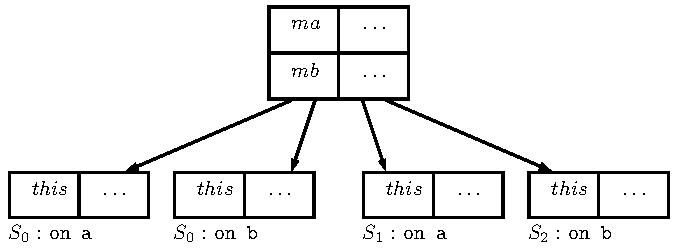
\includegraphics[scale=0.8]{figs/chapter_02_symtab_chain.pdf}
  \caption{Scoping structure of a synchroniser program using the zip2 synchroniser as an example}
  \label{fig:symtab_chain}
  \end{figure}

The symbol table implementation supports three operations: create new symbol table, put new entry in table and get entry for identifier from table. In the sequel, we refer to these operations as \emph{NewSymtab}(symtab), symtab.\emph{put}(\emph{ID, value}) and symtab.\emph{get}(\emph{ID}). The pseudo-code implementations of symtab.\emph{get} and symtab.\emph{put} are given in Fig. \ref{symtab_get} and Fig. \ref{symtab_put} respectively.

\begin{figure}%[h!]
\noindent\fbox{%
\begin{minipage}{\dimexpr\linewidth-2\fboxsep-2\fboxrule\relax}
\begin{algorithmic}[1]
\Function{get}{$symtab, id$}
  \While{$symtab \; is \; not \; nil$}
    \State $tmp\gets get(symtab, id)$
    \If{$tmp$}
      \State \textbf{return} \emph{tmp}
    \Else
      \State $symtab\gets previous(symtab)$\Comment{\emph{previous(symtab)} returns a symbol table of the most-closely outer scope}
    \EndIf
  \EndWhile
  \State \textbf{return} \emph{not\_found}
\EndFunction
\end{algorithmic}
\end{minipage}%
}
\caption{Getting an entry for an identifier from the chained symbol table\label{symtab_get}}
\end{figure}

The synchroniser language does not permit using of the reserved words (Appendix \ref{sync_kw}) as identifiers. This is checked before putting an identifier in the symbol table.

\begin{figure}%[h!]
\noindent\fbox{%
\begin{minipage}{\dimexpr\linewidth-2\fboxsep-2\fboxrule\relax}
\begin{algorithmic}[1]
\Function{put}{$symtab$, $id$, $value$}
  \If{\emph{id is reserved}}
    \State \emph{error}
  \EndIf
  \State $tmp\gets get(symtab, id)$
  \If{$not \; tmp$}
    \State $symtab\gets (id, value)$
  \Else
    \State \emph{error}
  \EndIf
\EndFunction
\end{algorithmic}
\end{minipage}%
}
\caption{Putting a new entry in the symbol table\label{symtab_put}}
\end{figure}



%Chaining of symbol tables results in a tree structure (probably we can simplity it somehow, because we do not really need a tree of scopes).

%The symbol table contains types and (possibly) locations. Builing of a symbol table Dragon book p.90.


\subsection{Static Analysis}
Static analysis includes:
\begin{itemize}
\item Semantic checking. Constraints such as an identifier is declared at most once in a scope
\item Type checking. The type rules of a language assure that an operator or function is applied to the right number and type of operands.
\end{itemize}

  \subsubsection*{Semantic checking}
In this section we describe the semantic checks that are not enforced by the grammar.

The synchroniser language requires identifiers except for state expression aliases to be declared before they are used. Moreover, an identifier must be declared at most once in a scope. The channels, on which the transitions in the synchroniser are made, must be declared in the channel signature as well as the channels where messages are sent. In order to check those, we maintain three symbol tables for identifiers, input channels and output channels. The scheme given in Fig. \ref{synt_scheme} shows how the symbol tables are managed and used during the syntax analysis. The symbol tables are initialised before the syntax analyser runs, as shown in Fig. \ref{symtab_init}.

The attribute \emph{type} is added to each entry in the symbol table. State variables are assigned type \emph{integer}. Non-integer variables, whose structure is unknown, are assigned a special type \emph{void}, which stands for a variable CAL term. A detailed information about the synchroniser language type system is provided in section \ref{type_check}.

\begin{figure}[h!]
\noindent\fbox{%
\begin{minipage}{\dimexpr\linewidth-2\fboxsep-2\fboxrule\relax}
\begin{algorithmic}
\Function{init}{}
    \State $InChantab\gets NewSymtab(nil)$
    \State $OutChantab\gets NewSymtab(nil)$
    \State $RootSymtab\gets NewSymtab(nil)$
\EndFunction
\end{algorithmic}
\end{minipage}%
}
\caption{Initialisation of symbol tables\label{symtab_init}}
\end{figure}



%\begin{figure}[h!]
\begin{sidewaystable}
\def\arraystretch{2} 
\begin{tabular*}{1\textwidth}{p{0.5\textwidth}|p{0.5\textwidth}}
\hline
Production & Semantic Action\\

\hline

\parbox{0.5\textwidth}{
\iangled{synch} ::= \tangled{synch} \iangled{ID} \tangled{(} \iangled{input} [\tangled{,} \iangled{input}]*

~~\tangled{|} \iangled{output} [\tangled{,} \iangled{output}]* \tangled{)} \tangled{\{} \iangled{decl}* \iangled{state}$^+$ \tangled{\}}
} & \parbox{0.5\textwidth}{
/* \emph{synch} is the abstract syntax tree of the source code.  */
}\\

\hline

\parbox{0.5\textwidth}{
\iangled{input} ::= \iangled{chan} [\tangled{:} (\iangled{ID} $\mid$ \iangled{NUMBER})]

\iangled{chan} ::= \iangled{ID}
} & \parbox{0.5\textwidth}{
\emph{foreach} \iangled{chan}

~~InChantab.\emph{put}(\iangled{chan}, \emph{type=void})
}\\

\hline

\parbox{0.5\textwidth}{
\iangled{output} ::= \iangled{chan} [\tangled{:} \iangled{depth\_exp}]

\iangled{chan} ::= \iangled{ID}
} & \parbox{0.5\textwidth}{
\emph{foreach} \iangled{chan}

~~OutChantab.\emph{put}(\iangled{chan}, \emph{type=void})
}\\

\hline

\parbox{0.5\textwidth}{
\iangled{decl} ::= \tangled{store} \iangled{store\_id\_list} \tangled{;}

~~$\mid$ \tangled{state} \iangled{type} \iangled{state\_id\_list} \tangled{;}

\iangled{store\_id\_list} ::= \iangled{id\_list}

\iangled{state\_id\_list} ::= \iangled{id\_list}
} & \parbox{0.5\textwidth}{
\emph{foreach} \texttt{id} \emph{in} \iangled{store\_id\_list}

~~Symtab.\emph{put}(\texttt{id}, \emph{type=void})

\emph{foreach} \texttt{id} \emph{in} \iangled{state\_id\_list}

~~Symtab.\emph{put}(\texttt{id}, \emph{type=int})
}\\

\hline

\parbox{0.5\textwidth}{
\iangled{trans\_stmt} ::=

~~\iangled{trans\_name} [\tangled{.} \iangled{condition}] [\tangled{\&} \iangled{int\_exp} ] \iangled{actions}
} &\\

\hline

\parbox{0.5\textwidth}{
\iangled{trans\_name} ::= \iangled{ID}
} & \parbox{0.5\textwidth}{
\emph{if not} InChantab.\emph{get}(\iangled{ID})

~~\emph{error}

Symtab = NewSymtab(\emph{RootSymtab})

Symtab.\emph{put}(\tangled{this}, \emph{type=void})
}\\

\hline

\parbox{0.5\textwidth}{
\iangled{condition} ::= \tangled{@} \iangled{segmark}

~~$\mid$ \tangled{?} \iangled{ID}

~~$\mid$ \tangled{else}

\iangled{segmark} ::= \iangled{ID}
} & \parbox{0.5\textwidth}{
\emph{if not} Symtab.\emph{get}(\iangled{segmark})

~~\emph{error}
}\\

\hline

\parbox{0.6\textwidth}{
\iangled{condition} ::= [\tangled{?} \iangled{ID}] \tangled{(} \iangled{id\_list} [\tangled{||} \iangled{tail} ]\tangled{)}
} & \parbox{0.4\textwidth}{
\emph{foreach} \texttt{id} \emph{in} \iangled{id\_list} $\cap$ \iangled{tail}

~~Symtab.\emph{put}(\texttt{id}, \emph{type=void})

tmp = Symtab.\emph{get}(\tangled{this})

tmp.\emph{type} = \texttt{\{ \tangled{$p_1$}:\emph{void}, \dots \tangled{$p_n$}:\emph{void} \}}, where \emph{$p_1$, \dots $p_n$} are elements of \iangled{id\_list}

\emph{if} \iangled{tail}

~~tmp.\emph{type} = tmp.\emph{type} $\mid$ \iangled{tail}
}\\

\hline

\parbox{0.5\textwidth}{
\iangled{send\_stmt} ::= \tangled{send} \iangled{dispatch} [\tangled{,} \iangled{dispatch}* \tangled{;}

\iangled{dispatch} ::= \iangled{msg\_exp} \tangled{=>} \iangled{ID}
} & \parbox{0.5\textwidth}{
tmp = OutChantab.\emph{get}(\iangled{ID})

\emph{if not} tmp

~~\emph{error}
}\\

\hline
% goto is a state list, not a chan list
%\parbox{0.5\textwidth}{
%\iangled{goto\_stmt} ::= \tangled{goto} \iangled{id\_list} \tangled{;}
%} & \parbox{0.5\textwidth}{
%\emph{foreach} \texttt{id} \emph{in} \iangled{id\_list}
%
%~~\emph{if not} InChantab.\emph{get}.(\texttt{id})
%
%~~~~\emph{error}
%}\\
%
%\hline

\end{tabular*}
\caption{Symbol tables management and duplicate declaration checking scheme\label{synt_scheme}}
\end{sidewaystable}
%\end{figure}

%Check if all gotos point to existing states
The synchroniser compiler checks if the transition diagram of a synchroniser is connected. The algorithm given in Fig. \ref{goto_check} walks the abstract syntax tree \emph{synch} and constructs two sets: the set of the synchroniser state labels \emph{StateSet} and the set of the goto labels \emph{GotoSet}. The set $GotoSet \setminus StateSet$ contains goto labels that point to non-existent states. If this set is not empty the compilation reporting an error. The set $StateSet \setminus (GotoSet \cup \tangled{start})$ contains unreachable states that are eliminated, also reporting an error. The algorithm also checks if the labels of the synchroniser states are unique.

A synchroniser program must have the state labeled \tangled{start}. The existence of this state is checked once the $StateSet$ is constructed.

\begin{figure}%[h!]
\noindent\fbox{%
\begin{minipage}{\dimexpr\linewidth-2\fboxsep-2\fboxrule\relax}
\begin{algorithmic}[1]
\Function{get\_states}{$synch$}
  \State $StateSet\gets []$
  \State $GotoSet\gets []$
  \For{\textbf{each} \emph{state in state\_list(sync)}}
    \If{$label(state) \in StateSet$}
      \State \emph{error}\Comment{The state label is not unique}
    \Else
      \State $s\gets s$ \textbf{..} $label(state)$
    \EndIf

    \For{\textbf{each} \emph{trans in trans\_list(state)}}
      \For{\textbf{each} \emph{gotostate in goto\_list(trans)}}
        \If{$gotostate \notin GotoSet$}
          \State $GotoSet\gets GotoSet$ \textbf{..} $gotostate$
        \EndIf
      \EndFor
    \EndFor
  \EndFor
  \State \textbf{return} \emph{(StateSet, GotoSet)}
\EndFunction
\end{algorithmic}
\end{minipage}%
}
\caption{Construction of \emph{StateSet} and \emph{GotoSet}\label{goto_check}}
\end{figure}


%The synchroniser language supports configurable channel depth for input and output channels. If an input channel has the configurable depth, the depth of an output channel may be specified as an integer shift to the input channel depth. In other cases the shift is not needed.

%Channel signature. If the output channel depth is in the form of depth expression $p+integer$, then $p$ should be the depth of one of the input channels. $p$ is not allowed anywhere in state expressions.
%  \begin{itemize}
%  \item (a:p | b:p+1) - allowed
%  \item (a:p | b:0) - allowed
%  \item (a:p | b:r) - allowed
%  \item (a:p | b:r+1) - NOT allowed
%  \end{itemize}
%The special depth $-1$ indicated that the channel is not used. Therefore, if it is an input channel, all the transitions reading from it can be removed. If it is an output channel, and the transition that sends to this channel is valid, then an error must occur.


The synchroniser language provides two types of state variable: an integer of the specified size and an enumeration. The size defines the value range of the integer. The value range of the enumeration is specified in the variable declaration. Fig. \ref{int_range} gives formulae for the value range computation.

%The width  decreases the number of possible states of a synchroniser. At low level state variables are machine- and target language- depedent integers.

\begin{figure}%[h!]
\centering
\begin{tabular}{|c|c|}
\hline
Type & Values\\
\hline
$int(n)$ & $[0; 2^{n}-1] \cap \mathbb{Z}$\\
\hline
$enum(a_1$, $a_2$, $\dots$ $a_n)$ & $[0; n-1] \cap \mathbb{Z}$\\
\hline
$enum(a_1=N_1$, $a_2=N_2$, $\dots$ $a_n=N_n)$ & $N_1$, $N_2$, $\dots$ $N_n$\\
\hline
\end{tabular}
\caption{Computing the value range of an integer variable\label{int_range}}
\end{figure}

For a state expression that evaluates to an integer we can check if the computed value belongs to the assignment-destination value-range. The symbol table stores the value-range information for integer entries and provides an interface to it in the form of boolean function \texttt{check\_range}(\emph{id}, \emph{value}). The function returns \emph{true} if the \emph{value} fits in the \emph{id} value range and \emph{false} otherwise. Fig. \ref{ts_stmt} shows how the check is integrated into the syntax analyser.

%Check if the range condition is valid at least for assignments (int(1) x = 10 is not good, should issue a warning, check what would be assigned to x in C). For the state expressions that evaluate during the execution of the synchroniser it's probably ok to delegate the overflow checks to the C compiler.


    \paragraph{Tests}
We have developed a test suite for the semantic analyser. It uses the standard python unit testing framework \emph{unittest}. The tests expand the abstract syntax tree into a nested list and compare the result with the expected value.


  \subsubsection*{Type checking}\label{type_check}
The design of the type checker is based on information about the syntactic constructs in the language, the notion of types and the rules for assigning types to language constucts. The type of a language construct is denoted by a type expression. Informally, a type expression is either a basic type or the application of an operator called a type constructor to other type expressions. A collection of rules for assigning type expressions to language constructs is called a type system.

The communication protocol of the \ak\ runtime system prototype supports only choices. When a synchroniser reads a message from its input channel, the record that belongs to the variant specified in the synchroniser transition is instantiated\footnote{this means that store variables cannot keep multiple variants}. We take this into account in implementing the type system of the synchroniser language. Because the synchronisers can read values only of the fields that are known to be integer, the basic types in the synchroniser language are integer and CAL variable. Integer is the type of state variable. CAL variables are building blocks for the only constructed type in the synchroniser language -- a record. A record is constructed by the concatenation of two records. The pseudo-code of the record constructor $||$ is given in Fig. \ref{rec_construc}. The record constructor is obviously commutative and associative.

\begin{figure}%[h!]
\noindent\fbox{%
\begin{minipage}{\dimexpr\linewidth-2\fboxsep-2\fboxrule\relax}
\begin{algorithmic}[1]
\Function{$||$}{$r_1, \; r_2$}
  \If{$len(r_1)\le len(r_2)$}
    \State $r_{iter}\gets r_1$
    \State $r\gets r_2$
  \Else
    \State $r_{iter}\gets r_2$
    \State $r\gets r_1$
  \EndIf\Comment{\emph{$r$ is the record that contains fewer label-value pairs}}

  \For{\textbf{each} \emph{label-value pair (l,v) in} $r_{iter}$}
    \If{$r(l)$}\Comment{\emph{if label l exists in r}}
      \State $r(l)\gets union(r(l),v)$
    \Else
      \State $r(l)\gets v$
    \EndIf
  \EndFor
  \State \textbf{return r}
\EndFunction
\end{algorithmic}
\end{minipage}%
}
\caption{The record type constructor $||$\label{rec_construc}}
\end{figure}

The case when a label-value pair labeled $l$ exists in both operand records $r_1$ and $r_2$ is indicated with $union(r_1(l),r_2(l))$. The CAL solver resolves which option to take during the constraint aggregation pass in the \ak\ compiler.
%When labels intersect, it is the deal for CAL solver to resolve with option to take (it should consider flow inheritance).

We describe the type systems in terms of grammar productions and corresponding semantic actions. The type systems for state and store expressions is given in Fig. \ref{ts_int_exp} and Fig. \ref{ts_data_exp} respectively. The synthesized attribute \emph{type} for an expression \iangled{E} gives the type of the expression assigned by the type system for the expression generated by \iangled{E}. The type system for statements is given in Fig. \ref{ts_stmt}. It assures that the left hand side can be assigned to.


\begin{figure}%[h!]
%\begin{sidewaystable}
\def\arraystretch{2} 
\begin{tabular*}{1\textwidth}{p{0.5\textwidth}|p{0.5\textwidth}}
\hline
Production & Semantic Action\\

\hline

\parbox{0.5\textwidth}{
\iangled{assign} ::= \iangled{dest} \tangled{=} \tangled{[} \iangled{int\_exp\_c} \tangled{]}

\iangled{dest} ::= \iangled{ID}
} & \parbox{0.5\textwidth}{
tmp = Symtab.\emph{get}(\iangled{dest})

\emph{if not} tmp

~~Symtab.\emph{put}(\iangled{dest}, \emph{type=int})

\emph{else}

~~\emph{if} tmp.\emph{type} != \emph{int}

~~~~\emph{error}

~~\emph{if} \iangled{int\_exp\_c} \emph{evaluates to int}

~~~~\emph{if not check\_range}(\iangled{dest}, \emph{eval}(\iangled{int\_exp\_c}))

~~~~~~\emph{error}
}\\

\hline

\parbox{0.5\textwidth}{
\iangled{assign} ::= \iangled{dest} \tangled{=} \iangled{data\_exp}

\iangled{data\_exp} ::=

~~(\iangled{data} $\mid$ \tangled{(} \iangled{data} \tangled{)})

} & \parbox{0.5\textwidth}{
tmp = Symtab.\emph{get}(\iangled{dest})

\emph{if not} tmp

~~\emph{error}

\emph{if} tmp.\emph{type == int}

~~\emph{error}

tmp.\emph{type} = \iangled{data\_exp}.\emph{type}
}\\

\hline

\end{tabular*}
\caption{Type system for statements\label{ts_stmt}}
%\end{sidewaystable}
\end{figure}



\begin{figure}%[h!]
%\begin{sidewaystable}
\def\arraystretch{2} 
\begin{tabular*}{1\textwidth}{p{0.5\textwidth}|p{0.5\textwidth}}
\hline
Production & Semantic Action\\

\hline

\parbox{0.5\textwidth}{
\iangled{int\_exp\_c} ::= \iangled{NUMBER} $\mid$ \iangled{ID}
} & \parbox{0.5\textwidth}{
tmp = Symtab.\emph{get}(\iangled{ID})

\emph{if not} tmp

~~\emph{error}

\emph{if} tmp.\emph{type != int}

~~\emph{error}

\iangled{int\_exp\_c}.\emph{type} = \emph{int}
}\\

\hline

\parbox{0.5\textwidth}{
\iangled{int\_exp\_c} ::= \tangled{(} \iangled{$int\_exp\_c_{1}$} \tangled{)}

~~$\mid$ \tangled{-} \iangled{$int\_exp\_c_{1}$}

~~$\mid$ \tangled{!} \iangled{$int\_exp\_c_{1}$}
} & \parbox{0.5\textwidth}{
\iangled{int\_exp\_c}.\emph{type} = \iangled{$int\_exp\_c_{1}$}.\emph{type}
}\\

\hline

\parbox{0.5\textwidth}{
\iangled{int\_exp\_c} ::=

~~~~\iangled{$int\_exp\_c_{1}$} \iangled{op} \iangled{$int\_exp\_c_{2}$}

\iangled{op} ::= \tangled{+} $\mid$ \tangled{-} $\mid$ \tangled{*} $\mid$ \tangled{/} $\mid$ \tangled{\%}

~~$\mid$ \tangled{<<} $\mid$ \tangled{>>} $\mid$ \tangled{|} $\mid$ \tangled{\&} $\mid$ \tangled{\textasciicircum}

~~$\mid$ \tangled{<} $\mid$ \tangled{>} $\mid$ \tangled{==} $\mid$ \tangled{!=} $\mid$\tangled{<=}

~~$\mid$ \tangled{>=} $\mid$ \tangled{\&\&} $\mid$ \tangled{||}
} & \parbox{0.5\textwidth}{
\emph{if} \iangled{$int\_exp\_c_{1}$}.\emph{type} == \emph{int}

~~\emph{and} \iangled{$int\_exp\_c_{2}$}.\emph{type} == \emph{int}

~~\iangled{int\_exp\_c}.\emph{type} = \emph{int}

\emph{else}

~~\emph{error}
}\\

\hline

\end{tabular*}
\caption{Type system for state expressions\label{ts_int_exp}}
%\end{sidewaystable}
\end{figure}


\begin{figure}%[h!]
%\begin{sidewaystable}
\def\arraystretch{2} 
\begin{tabular*}{1\textwidth}{p{0.5\textwidth}|p{0.5\textwidth}}
\hline
Production & Semantic Action\\

\hline

\parbox{0.5\textwidth}{
\iangled{data} ::= \iangled{item\_list}

\iangled{item\_list} ::= \iangled{item} [\tangled{||} \iangled{item}]*
} & \parbox{0.5\textwidth}{
\emph{foreach} \texttt{item} \emph{in} \iangled{item\_list}

~~\iangled{data}.\emph{type} = \iangled{data}.\emph{type} $||$ \texttt{item}.\emph{type}
}\\

\hline

\parbox{0.5\textwidth}{
\iangled{item} ::= \tangled{this}
} & \parbox{0.5\textwidth}{
tmp = Symtab.\emph{get}(\tangled{this})

\iangled{item}.\emph{type} = tmp.\emph{type}
}\\

\hline

\parbox{0.5\textwidth}{
\iangled{item} ::= \iangled{ID}
} & \parbox{0.5\textwidth}{
tmp = Symtab.\emph{get}(\iangled{ID})

\emph{if not} tmp

~~\emph{error}

\emph{if} tmp.\emph{type == int}

~~\emph{error}

\iangled{item}.\emph{type} = tmp.\emph{type}
}\\

\hline

\parbox{0.5\textwidth}{
\iangled{item} ::= \tangled{'} \iangled{ID}
} & \parbox{0.5\textwidth}{
tmp = Symtab.\emph{get}(\iangled{ID})

\emph{if not} tmp

~~\emph{error}

\iangled{item}.\emph{type} = \{ \tangled{ID}:tmp.\emph{type} \}
}\\

\hline

\parbox{0.5\textwidth}{
\iangled{item} ::= \iangled{ID} \tangled{:} \iangled{rhs}

\iangled{rhs} ::= \iangled{int\_exp} $\mid$ \iangled{rhs\_ID}

\iangled{rhs\_ID} ::= \iangled{ID}
} & \parbox{0.5\textwidth}{
\emph{if} \iangled{rhs\_ID}

~~tmp = Symtab.\emph{get}(\iangled{rhs\_ID})

~~\emph{if not} tmp

~~~~\emph{error}

tmp = Symtab.\emph{get}(\iangled{ID})

\iangled{item}.\emph{type} = \{ \tangled{ID}:\iangled{rhs}.\emph{type} \}
}\\

\hline

\end{tabular*}
\caption{Type system for store expressions\label{ts_data_exp}}
%\end{sidewaystable}
\end{figure}

%If an identifier was met and it is already in the current scope of symbol table, it must have the same type (int or data) as before.


%\subsection{Code optimisation}
%Code optimiser is a framework for writing optimisation passes, which currently has only dead code elimination. 
%
%  \paragraph{Dead code elimination}
%\begin{itemize}
%\item Remove unreachable states of an automaton (when there's no state variables involved).
%
%\item Remove unreachable transitions based on Section Execution order.
%
%\item Remove unused state, store variables and assignments (this may require some simple def-use analysis, probably can put it into symbol tables).
%\end{itemize}


\subsection{Code Generation}
  \subsubsection*{Synchroniser runtime code}
The compiler generates a data structure that is passed to the \ak\ runtime system for the interpretation.


  \subsubsection*{Synchroniser passport}
Synchronisers rely on both TPL and CAL for their definition. The CAL aspects of a synchroniser are confined to the CAL terms for its input and output channels. Those terms are not straightforward since they have to be fairly generic to match the broadest possible formats of producer and consumer messages involved in the act of synchronisation. On the other hand, the synchroniser passport is produced solely on the basis of the synchroniser code, exclusively by program analysis; the programmer does not supply an explicit passport for this.

The first thing that requires CAL is the input interface. As mentioned above, the communication protocol of the \ak\ runtime system prototype supports only choices. The use of a variant on a channel in any transition on that channel immediately associates the \emph{choice} term structure with it. For example, a channel $a$ that is tested on variants \textbf{?}\emph{v} and \textbf{?}\emph{w} in transitions has a term comparable with \textbf{(:} \tangled{v}:\emph{\$vterm}, \tangled{w}:\emph{\$wterm} $||$ \emph{\$tail} \textbf{:)}, where the variables \emph{\$vterm} and \emph{\$wterm} represent the terms for variants \emph{v} and \emph{w} and \emph{\$tail} represents the choice term that contains the rest of the variants. If a choice is known to carry a single variant, the variant is labeled \emph{uniq}. A transition that does not specify a variant label expects a unique message variant.

The symbol table for a transition maintains a special entry \tangled{this}. It holds the term of the message accepted by the transition. The algorithm in Fig. \ref{input_term} walks the synchroniser transitions and constructs the CAL input term for the synchroniser\footnote{The algorithm relies on the abstract syntax tree structure (see Appendix. \ref{ast_app})}.

\begin{figure}%[h!]
\noindent\fbox{%
\begin{minipage}{\dimexpr\linewidth-2\fboxsep-2\fboxrule\relax}
\begin{algorithmic}[1]
\Function{input\_term}{$synch$}
  \State $CondDict\gets nil$

  \For{\textbf{each} \emph{state in state\_list(sync)}}
    \For{\textbf{each} \emph{trans in trans\_list(state)}}
      \State $cond\gets get\_condition(trans)$
      \If{$port \in CondDict$}
        \State $CondDict(port)\gets CondDict(port)$ \textbf{..} $cond$
      \Else
        \State $CondDict\gets CondDict$ \textbf{..} $(port,\:cond)$
      \EndIf
    \EndFor
  \EndFor

  \State $InputTerm\gets nil$

  \For{\textbf{each} \emph{(port,cond\_set) in CondDict}}
    \State $PortTerm\gets nil$

    \For{\textbf{each} \emph{cond in cond\_set}}
      \State $variant\gets get\_variant(cond)$
      \State $this\gets$ Symtab.\emph{get}(\tangled{this})
      
      \If{\emph{variant is unique}}
        \If{$PortTerm \neq nil$}
          \emph{error}
        \EndIf
        \State $PortTerm\gets$ \textbf{(:} \tangled{uniq}:\emph{this} \textbf{:)}
        \State \textbf{break}
      \Else
        \State $PortTerm\gets PortTerm \; || \; this$
      \EndIf
    \EndFor

    \State $InputTerm\gets InputTerm$ \textbf{..} $(port,\:PortTerm)$
  \EndFor

  \State \textbf{return} \emph{InputTerm $||$ \emph{\$tail}}
\EndFunction
\end{algorithmic}
\end{minipage}%
}
\caption{Construction of the synchroniser input term\label{input_term}}
\end{figure}

Since a choice is in fact a collection of label-record pairs, the constructor $||$ (Fig. \ref{rec_construc}) can be applied for choices. When \emph{InputTerm} contains a label-value pair (\tangled{v},\:$value$) and the label \tangled{v} occurs in another transition, the union $||$ of these two choices results in the following:
\begin{IEEEeqnarray}{rCl}
& union \: (\textbf{(:}\: \tangled{v}:\$vterm_1 \;|\; \$tail_1 \:\textbf{:)}, \; \textbf{(:}\: \tangled{v}:\$vterm_2 \;|\; \$tail_2 \:\textbf{:)})\nonumber\\
=& \textbf{(:}\: \tangled{v}:union \: (\$vterm_1,\:\$vterm_2) \;|\; (\$tail_1 \;||\; \$tail_2) \:\textbf{:)}\nonumber
\end{IEEEeqnarray}


Now consider the output interface. The algorithm in Fig. \ref{output_term} collects the dispatches for every output channel and combines them into the output term of every output channel.

\begin{figure}%[h!]
\noindent\fbox{%
\begin{minipage}{\dimexpr\linewidth-2\fboxsep-2\fboxrule\relax}
\begin{algorithmic}[1]
\Function{output\_term}{$synch$}
  \State $DispatchDict\gets nil$

  \For{\textbf{each} \emph{state in state\_list(sync)}}

    \For{\textbf{each} \emph{trans in trans\_list(state)}}
      \State $send\gets get\_send(trans)$
      \State $(msg,\:port)\gets (get\_msg(send),\:get\_port(send)$
      \If{$port \in DispatchDict$}
        \State $DispatchDict(port)\gets DispatchDict(port)$ \textbf{..} $msg$
      \Else
        \State $DispatchDict\gets DispatchDict$ \textbf{..} $(port,\:msg)$
      \EndIf
    \EndFor
  \EndFor

  \State $OutputTerm\gets nil$

  \For{\textbf{each} \emph{(port,msg\_set) in DispatchDict}}
    \State $PortTerm\gets nil$
    \For{\textbf{each} \emph{msg in msg\_set}}
      \If{\emph{msg is MsgData}}\Comment{\emph{msg matches} [\tangled{?}\iangled{ID}]\iangled{data}}
        \State $(variant,\:data)\gets (get\_variant(msg),\:get\_data(msg))$
        \For{\textbf{each} \emph{item in data}}
          \If{\emph{item is ItemVar or item is ItemPair}}\Comment{\emph{item is either 'id or id:value}}
            \State $(lhs,\:rhs)\gets expand(item)$
            \State $PortTerm\gets PortTerm \;||\; $\textbf{\{}\emph{lhs:type(rhs)}\textbf{\}}
          \Else\Comment{\emph{item is either this or id}}
            \State $PortTerm\gets PortTerm \;||\; type(id)$
          \EndIf
        \EndFor
      \EndIf
    \EndFor
    \State $OutputTerm\gets OutputTerm$ \textbf{..} $(port,\:PortTerm)$
  \EndFor

  \State \textbf{return} \emph{OutputTerm $||$ \emph{\$tail}}
\EndFunction
\end{algorithmic}
\end{minipage}%
}
\caption{Construction of the synchroniser output term\label{output_term}}
\end{figure}

The function $type(id)$ performs the symbol table lookup and returns the \emph{type} attribute value for the \tangled{id} entry.


\section{Discussion and Future Work}
In this chapter we have presented the language for \ak\ synchronisers. We have developed the language compiler that generates the CAL passport of the synchroniser. The message format in \ak\ is based on the Message Definition Language (MDL) with the restriction that data on streams are organised as collections of alternative records of label-value pairs. A value in a record can have any structure that is allowed by the MDL. The synchroniser that we have presented matches only a top-level structure of a message. The MDL generates a much broader set of terms than the current version synchroniser can synchronise; however, it needs to be elaborated whether the implementation of lower level synchronisation in synchronisers is useful for the real world applications.

The current version of the language does not define flow inheritance in synchronisers. The synchroniser \emph{code} only needs to access the label-value parts of the message it matches. Thus, the flow inheritance should be supported outside of the synchroniser definition and the question how it should be done is left open.

The compiler we have implemented does not optimise the code deeply. We have only implemented an elimination of unused states. However, a broader set of dead code elimination optimisations can be implemented\footnote{E.g. a conditional transition can be eliminated if its condition always evaluates to \emph{false}}.

